\documentclass[12pt,a4paper]{extarticle}
\usepackage[left=3cm,right=2cm,top=2cm,bottom=2cm,headheight=18pt]{geometry}
\usepackage{fontspec}
\setmainfont{Liberation Serif}
\setsansfont{Liberation Serif}
\setmonofont{Liberation Mono}
\usepackage{unicode-math}
\setmathfont{texgyretermes-math.otf}
\usepackage{amsmath,graphicx,booktabs,longtable,array,enumitem}
\usepackage{pgfplots}
\usepgfplotslibrary{groupplots}
\pgfplotsset{compat=1.17,every axis/.append style={font=\fontsize{11bp}{13.2bp}\selectfont}}
\usepackage{titlesec,fancyhdr}
\usepackage[hidelinks,unicode]{hyperref}
\usepackage{url}
\urlstyle{same}
\setlength{\parindent}{1.27cm}
\setlength{\parskip}{0pt}
\linespread{1}
\setlength{\emergencystretch}{2em}
\clubpenalty=10000
\widowpenalty=10000
\titleformat{\section}{\normalfont\bfseries}{\thesection.}{0.5em}{}
\titleformat{\subsection}{\normalfont\bfseries}{\thesubsection.}{0.5em}{}
\titlespacing*{\section}{0pt}{1.2em}{0.5em}
\titlespacing*{\subsection}{0pt}{0.9em}{0.3em}
\setlist{nosep,leftmargin=1.27cm}
\pagestyle{fancy}
\fancyhf{}
\renewcommand{\headrulewidth}{0pt}
\renewcommand{\footrulewidth}{0pt}
\fancyhead[C]{\ifnum\value{page}>1\thepage\fi}
% Current statutory geometry/size baseline: O‘RQ-682 appendix §§43–51.
\newcolumntype{L}[1]{>{\raggedright\arraybackslash}p{#1}}
\begin{document}
\begin{flushright}Material 3\end{flushright}
\begin{center}
\textbf{SCIENTIFIC AND LEGAL JUSTIFICATION}\par
\textbf{of the proposals for inclusion in the draft normative legal act being prepared to implement paragraph 14 of Decree of the President of the Republic of Uzbekistan No. PF-193 of 11 September 2026}\par
\medskip
Abduxoliq Akmal ugli Ashuraliyev, independent researcher (ORCID 0009-0003-5482-5526)\par
Edition of 1 October 2026; calculations use the legal texts in force on 30 September 2026. English companion translation; the Russian edition is primary.
\end{center}

\section{Subject, legal basis and research question}
Subparagraph “a” of paragraph 13 of Decree PF-193 introduces from 1 January 2027 a multidimensional assessment that takes into account, in addition to the family’s financial condition, chronic illness, disability, external labour migration and large family size; subparagraph “b” provides for point-based scoring and assignment of families to categories; paragraph 14 instructs the National Agency for Social Protection under the President of the Republic of Uzbekistan (hereinafter, the Agency), jointly with the Ministry of Economy and Finance, to submit the draft act to the Presidential Administration by 1 December 2026\cite{ref1}. Financial condition remains one dimension of the assessment, so the income calculation rules of the Regulation on the Procedure for Maintaining the Social Registry (Annex 1 to Cabinet of Ministers Resolution No. 35 of 29 January 2026) continue to determine the result until replaced\cite{ref2}.

Decisions on Registry inclusion and category are made by the information module “automatically” (stage 6 of Annex 1 to the Regulation)\cite{ref2}. In such a system a family’s result is determined by how the software executes each threshold, equality to it, exceptions, units and periods. Article 24 of the Law “On Personal Data” requires the data subject to be told how an automated decision is made and its legal consequences, and an objection to be considered within ten days\cite{ref9}.

The research question is stated so that it can be refuted: \textbf{do the published income and category rules give a single, internally consistent result at the thresholds and throughout the declared input domain?} The finding is refuted by an error in transcribing a rule, an omitted applicable exception, a narrower lawful input domain or a disagreement with independent arithmetic.

\section{Sources and data}
Official texts of the acts on lex.uz as of 30 September — 1 October 2026 were used: Decree PF-193, Resolution No. 35 (consolidated with amendments of 22 May and 21 July 2026), Decree PF-258, and the Laws “On Normative Legal Acts”, “On Personal Data” and “On Appeals of Individuals and Legal Entities”\cite{ref1,ref2,ref3,ref7,ref9,ref20}. Resolution No. 35 and Decree PF-193 are officially published in the state language; amendment wording follows the Uzbek text.

Monthly minimum consumption expenditure per person in 2026 is $P=715{,}000$ soum\cite{ref5}; the minimum wage from 1 September 2026 is $M=1{,}360{,}000$ soum\cite{ref4}.

Two sources describe practice. On 17 July 2026 the Government portal reported that in 184 mahallas all 2,000 applications received in one month were refused without grounds, that appeals to the President on Registry inclusion rose from 30,000 to 46,000, and that the Prosecutor General’s Office was instructed to exercise strict oversight\cite{ref28}. The World Bank’s 2026 poverty and equity assessment states that the targeting formula was revised in early 2026 and that an assessment of its effectiveness is not yet available\cite{ref11}.

International experience supports the chosen mechanisms. Chile’s Ministry of Social Development and Family publishes the procedure for calculating the socio-economic rating with worked examples, “equal to or greater than” thresholds and a precedence rule when several checks are triggered\cite{ref32}. The World Bank notes that outdated registry data lead to inclusion and exclusion errors and that grievance redress mechanisms enhance transparency and accountability\cite{ref12}.

\section{Method}
\subsection{Objects and units}
Let $Y$ be the family’s counted income over three months and $N$ the counted number of members; monthly income per person is $D=Y/(3N)$ (point 18 of the Regulation). The formulas for individual income contributions and the category conditions are checked; full aggregation of $Y$ from administrative data is not reproduced. The September 2026 value of $M$ is used only in dated single-month calculations.

Calculations are performed by the reference program (electronic supplement). Numbers are entered as integers or strings of decimal and rational numbers; exact rational arithmetic is used, so equality comparisons are not distorted by binary rounding. Floating-point numbers, invalid divisors and incomplete data are rejected.

\subsection{Prespecified plan and case selection}
The list of checks and the case grids were fixed in the analysis plan before calculations were run. Income grid: $P$, $1.5P$, $2P$ with offsets of $-1$, $0$, $+1$ soum. Difficult life circumstances: values around $P$, $4P/3$, $1.5P$, $2P$. Land formula: all integer building areas $QM$ from $0$ to $UM$ for $UM=100$, $1{,}000$, $1{,}001$, $2{,}000$ m² (4,105 cases in total). Remittances: an unknown value and values around $2M$ for both country groups under two possible comparison periods. Tax base, self-employment and goats: prespecified points.

The grids are constructed domains, not a sample of families. The number of violating cases in a grid characterises the formula’s domain, not the share of families in Uzbekistan; shares of families can be determined only on the Agency’s data (Section~\ref{sec:agency}).

\subsection{Legal computational conditions}
Subpoint “a” of point 33 refuses recognition as a “state-supported family” or “poor family” where $D>P$; point 32 recognizes the family where there is no refusal ground; subpoints “a” and “b” of point 39 and point 3 of Decree PF-258 assign families with $D<P$ to these categories\cite{ref2,ref3}.

For difficult life circumstances $A=3D/4$. Points 34–35 of the Regulation allow inclusion in the “family at the poverty boundary” category where $D>P$ and $A\le1.5P$; subpoint “v” of point 39 and subpoint “v” of point 3 of Decree PF-258 describe this category by the interval from $P$ to $1.5P$. Both readings of the interval were checked: by ordinary and by reduced income.

Household plot area (point 27): $TEM=UM-QM-\min(0.2\,UM;\,200)$ m² over the domain $0\le QM\le UM$; monthly normative income $TEM\cdot0.035\,M\cdot k/100$, where 100 m² is one sotix and $k$ the mahalla land-tax coefficient. The calculations take $k=1$ because actual mahalla coefficients were not used; for another $k$ the amounts are multiplied by $k$.

Remittances (point 26): if the amount of transfers is not determined or is less than $2M$, normative income $cM$ applies, where $c=3$ for countries listed in Annex 6 and $c=2$ for other countries. Because the comparison period is not stated, both readings were calculated: comparison of a monthly amount $q$ and of a three-month total.

\subsection{Verification of results}
Results were verified in four ways: reproduction of the official example in point 30; manual inequalities; a separate checking program that does not use the calculation module and recomputes all 4,105 land cases, 12 hardship cases, 24 tax cases, 16 remittance cases and 6 goat cases with integer expressions; and automated tests. All 39 tests pass (29 checks of calculation rules and 10 provenance checks that reject an outdated, altered or incomplete result).

\section{Results}
\subsection{Official example and equality to the threshold}
The example in point 30 of the Regulation gives $6{,}480{,}000/(5\cdot3)=\mathbf{432{,}000}$ soum per person per month; the difference from the published answer is zero.

At $D=P=715{,}000$ both conditions $D>P$ and $D<P$ are false. The refusal ground of subpoint “a” of point 33 does not apply and, absent other refusal grounds, the family is recognized under point 32, but it does not satisfy the condition of categories “a” and “b” of point 39. A first-time applicant without a “mahalla seven” recommendation is assigned to no category. The control case of a family previously removed from a primary category falls, at $D=P$, within the interval of subpoint “v” of point 39, confirming that the cases are correctly separated.

The proposed amendment of subpoint “a” of point 33 (“equal to or higher” instead of “higher”) closes this case without amending Decree PF-258: the refusal condition becomes the exact complement of the category condition $D<P$ in point 3 of the Decree.

\subsection{Difficult life circumstances: inconsistency under either reading}
The conditions of the special procedure simplify exactly:
\begin{equation}
D>P,\quad\frac34D\le\frac32P\quad\Longleftrightarrow\quad P<D\le2P.
\end{equation}
If the interval of subpoint “v” of point 39 applies to ordinary income, families with $1.5P<D\le2P$ fall outside the special procedure; example: $D=1{,}287{,}000$ soum ($1.8P$). If the interval applies to reduced income, the condition $A\ge P$ is equivalent to $D\ge4P/3$, and families with $P<D<4P/3$ fall outside; example: $D=858{,}000$ soum ($1.2P$), reduced income $643{,}500<P$. Neither reading reproduces point 35 in full (Figure 1). At $P=715{,}000$: $4P/3=2{,}860{,}000/3$, $1.5P=1{,}072{,}500$, $2P=1{,}430{,}000$ soum.

\begin{center}
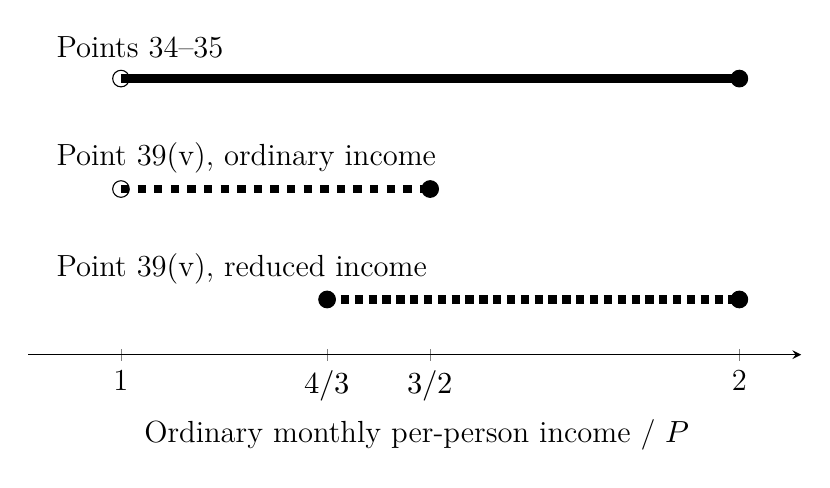
\begin{tikzpicture}
\begin{axis}[width=.94\linewidth,height=6cm,xmin=.85,xmax=2.1,ymin=.5,ymax=3.65,xtick={1,1.333333333,1.5,2},xticklabels={1,$4/3$,$3/2$,2},ytick=\empty,axis y line=none,axis x line=bottom,xlabel={Ordinary monthly per-person income / $P$}]
\addplot[black,line width=3pt] coordinates {(1,3)(2,3)};
\addplot[black,line width=3pt,dashed] coordinates {(1,2)(1.5,2)};
\addplot[black,line width=3pt,dotted] coordinates {(1.333333333,1)(2,1)};
\addplot[only marks,mark=*,mark size=3pt] coordinates {(2,3)(1.5,2)(1.333333333,1)(2,1)};
\addplot[only marks,mark=o,mark size=3pt,mark options={fill=white}] coordinates {(1,3)(1,2)};
\node[anchor=west] at (axis cs:.88,3.28) {Points 34–35};
\node[anchor=west] at (axis cs:.88,2.28) {Point 39(v), ordinary income};
\node[anchor=west] at (axis cs:.88,1.28) {Point 39(v), reduced income};
\end{axis}\end{tikzpicture}
\end{center}
\textbf{Figure 1.} Income normalised by $P$. A filled endpoint is included, an open one excluded. The top line shows the income conditions of points 34–35; the middle and bottom lines their intersection with the interval of subpoint “v” of point 39 under the two readings. The special procedure also requires the relevant circumstances, a recommendation and compliance with the quota.

\subsection{Negative area in the land formula}
For $UM\le1{,}000$ the formula equals $TEM=0.8\,UM-QM$ and is negative exactly when $QM>0.8\,UM$; for $UM>1{,}000$ it equals $TEM=UM-QM-200$, negative when $QM>UM-200$. The smallest value over $0\le QM\le UM$ is $-\min(0.2\,UM;200)$ m². Enumeration of 4,105 integer cases confirms the inequalities: 620 cases give a negative area (Table 1, Figure 2).

\begingroup\fontsize{11bp}{13.2bp}\selectfont
\begin{longtable}{p{\dimexpr\linewidth/5-2\tabcolsep\relax} p{\dimexpr\linewidth/5-2\tabcolsep\relax} p{\dimexpr\linewidth/5-2\tabcolsep\relax} p{\dimexpr\linewidth/5-2\tabcolsep\relax} p{\dimexpr\linewidth/5-2\tabcolsep\relax}}
\toprule
Plot $UM$ (m²) & Integer test cases & Negative cases & Minimum $TEM$ (m²) & Maximum floor change (soum/month) \\
\midrule
\endhead
100 & 101 & 20 & -20 & 9,520 \\
1,000 & 1,001 & 200 & -200 & 95,200 \\
1,001 & 1,002 & 200 & -200 & 95,200 \\
2,000 & 2,001 & 200 & -200 & 95,200 \\
Total constructed grid & 4,105 & 620 & — & — \\
\bottomrule
\end{longtable}
\endgroup
\textbf{Table 1.} Calculation at $M=1{,}360{,}000$ and $k=1$. Counts refer to the constructed grid. The last column is the largest change in the family’s monthly normative income when the zero floor is introduced.

Example: $UM=100$, $QM=90$ gives $TEM=-10$ m² and $-4{,}760$ soum of monthly normative income; a fully built-up 1,000 m² plot gives $-200$ m² and $-95{,}200$ soum. The negative contribution reduces the family’s counted income, although an area cannot physically be negative. The proposed zero floor gives $TEM=0$ and does not change the result where $TEM\ge0$.

\begin{center}
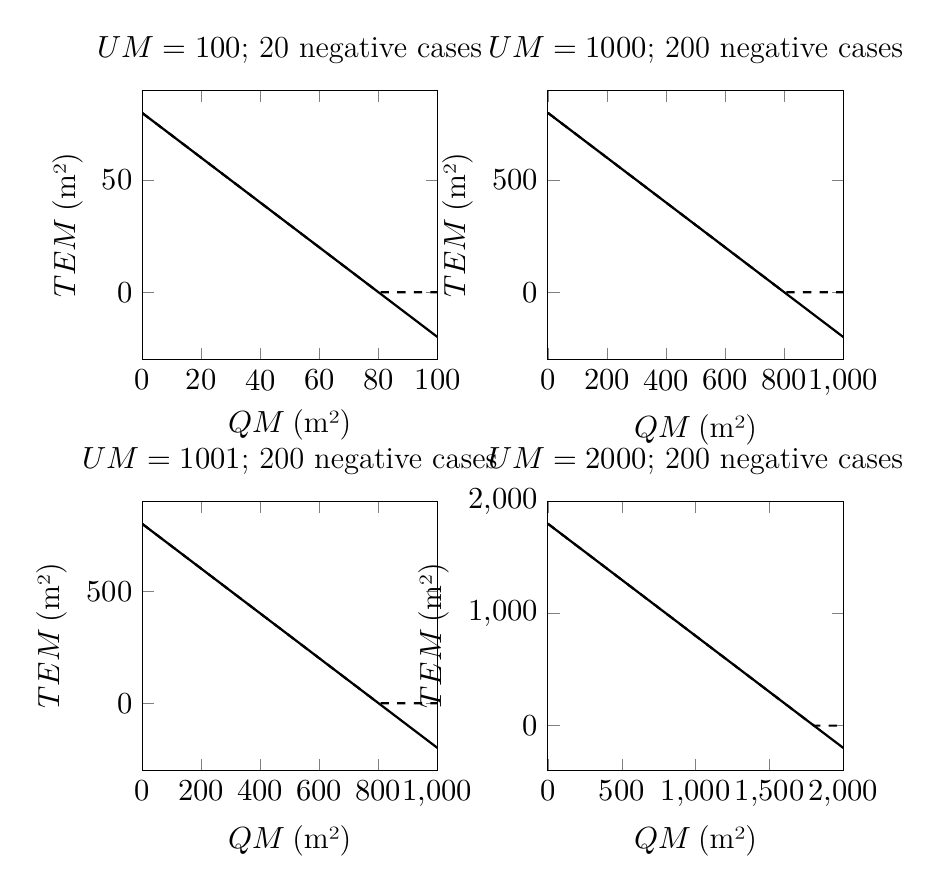
\begin{tikzpicture}
\begin{groupplot}[group style={group size=2 by 2,horizontal sep=1.4cm,vertical sep=1.8cm},width=.44\linewidth,height=5cm,xlabel={$QM$ (m²)},ylabel={$TEM$ (m²)},scaled ticks=false]
\nextgroupplot[title={$UM=100$; 20 negative cases},xmin=0,xmax=100]
\addplot[black,thick] coordinates {(0,80)(100,-20)};
\addplot[black,dashed,thick] coordinates {(0,80)(80,0)(100,0)};
\nextgroupplot[title={$UM=1000$; 200 negative cases},xmin=0,xmax=1000]
\addplot[black,thick] coordinates {(0,800)(1000,-200)};
\addplot[black,dashed,thick] coordinates {(0,800)(800,0)(1000,0)};
\nextgroupplot[title={$UM=1001$; 200 negative cases},xmin=0,xmax=1001]
\addplot[black,thick] coordinates {(0,801)(1001,-200)};
\addplot[black,dashed,thick] coordinates {(0,801)(801,0)(1001,0)};
\nextgroupplot[title={$UM=2000$; 200 negative cases},xmin=0,xmax=2000]
\addplot[black,thick] coordinates {(0,1800)(2000,-200)};
\addplot[black,dashed,thick] coordinates {(0,1800)(1800,0)(2000,0)};
\end{groupplot}\end{tikzpicture}
\end{center}
\textbf{Figure 2.} Solid line: current formula; dashed line: with the zero floor; for each $UM$ all integer $QM$ from $0$ to $UM$ are considered.

\subsection{Remittances: counted income falls as the transfer rises}
Equality $q=2M$ does not satisfy “less than $2M$”. Under the monthly reading, for countries in Annex 6 counted income falls from $3M$ just below the threshold to $2M$ at the threshold: a transfer of $2{,}719{,}999$ soum is counted as $4{,}080{,}000$, a transfer of $2{,}720{,}000$ as $2{,}720{,}000$. A one-soum rise in the transfer reduces counted income by $1{,}360{,}000$ soum. For other countries the monthly reading is continuous. Under the three-month-total reading, jumps arise for both groups (Table 2, Figure 3).

\begingroup\fontsize{11bp}{13.2bp}\selectfont
\begin{longtable}{p{\dimexpr\linewidth/4-2\tabcolsep\relax} p{\dimexpr\linewidth/4-2\tabcolsep\relax} p{\dimexpr\linewidth/4-2\tabcolsep\relax} p{\dimexpr\linewidth/4-2\tabcolsep\relax}}
\toprule
Conditional period & Country group & Monthly contribution drop (soum) & Per-person drop, four members (soum) \\
\midrule
\endhead
Monthly & Listed countries & 1,360,000 & 340,000 \\
Monthly & Other countries & 0 & 0 \\
Three-month total & Listed countries & 9,520,000/3 & 2,380,000/3 \\
Three-month total & Other countries & 5,440,000/3 & 1,360,000/3 \\
\bottomrule
\end{longtable}
\endgroup
\textbf{Table 2.} Fall in counted monthly income at the threshold, soum. Rows correspond to the two possible readings of the rule.

\begin{center}
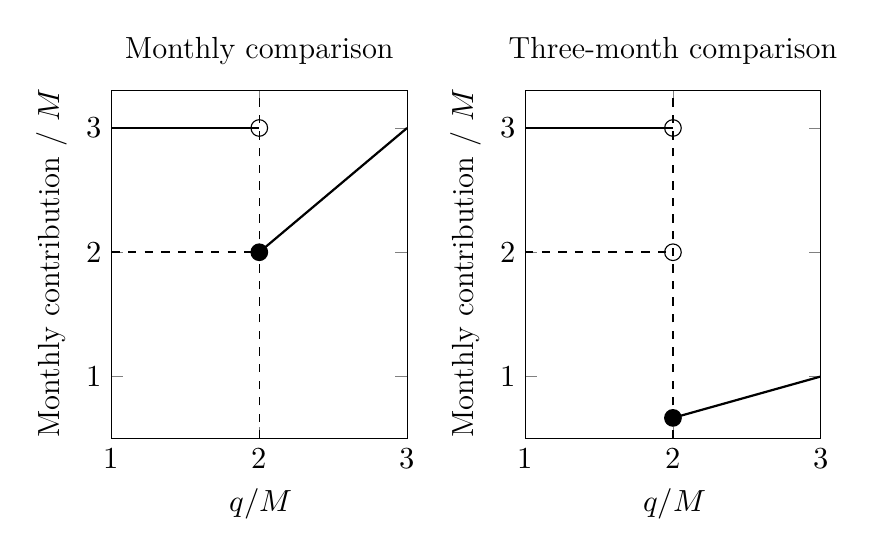
\begin{tikzpicture}
\begin{groupplot}[group style={group size=2 by 1,horizontal sep=1.5cm},width=.44\linewidth,height=6cm,xmin=1,xmax=3,ymin=.5,ymax=3.3,xtick={1,2,3},ytick={1,2,3},xlabel={$q/M$},ylabel={Monthly contribution / $M$}]
\nextgroupplot[title={Monthly comparison}]
\addplot[black,thick] coordinates {(1,3)(2,3)};
\addplot[black,dashed,thick] coordinates {(1,2)(2,2)};
\addplot[black,dashed] coordinates {(2,.5)(2,3.3)};
\addplot[black,thick] coordinates {(2,2)(3,3)};
\addplot[only marks,mark=*,mark size=3pt] coordinates {(2,2)};
\addplot[only marks,mark=o,mark size=3pt,mark options={fill=white}] coordinates {(2,3)};
\nextgroupplot[title={Three-month comparison}]
\addplot[black,thick] coordinates {(1,3)(2,3)};
\addplot[black,dashed,thick] coordinates {(1,2)(2,2)};
\addplot[black,dashed] coordinates {(2,.5)(2,3.3)};
\addplot[black,thick] coordinates {(2,.666666667)(3,1)};
\addplot[only marks,mark=*,mark size=3pt] coordinates {(2,.666666667)};
\addplot[only marks,mark=o,mark size=3pt,mark options={fill=white}] coordinates {(2,3)(2,2)};
\end{groupplot}\end{tikzpicture}
\end{center}
\textbf{Figure 3.} Horizontal axis: $q/M$; vertical axis: counted monthly income relative to $M$. Solid horizontal segments: countries in Annex 6; dashed: other countries; vertical line: threshold.

The proposed wording (Material 1, Section II, point 1) applies normative income where the monthly average of transfers is below the applicable normative income. Counted income equals $\max(q;\,cM)$ and does not decrease as $q$ rises; this is checked by an automated test on a 1,000-soum grid for both country groups. For other countries ($c=2$) the result coincides with the current monthly reading. Under both readings of the current rule, the proposed wording reduces no family’s counted income.

\subsection{Self-employment coefficients, tax base and livestock}
Point 23 sets eight coefficients of monthly normative income for the self-employed: four territory types and two sexes. The difference between the male and female coefficient in each territory equals $0.4M=544{,}000$ soum per month (Table 3). The calculation reflects normative income, not actual earnings.

\begingroup\fontsize{11bp}{13.2bp}\selectfont
\begin{longtable}{p{\dimexpr\linewidth/5-2\tabcolsep\relax} p{\dimexpr\linewidth/5-2\tabcolsep\relax} p{\dimexpr\linewidth/5-2\tabcolsep\relax} p{\dimexpr\linewidth/5-2\tabcolsep\relax} p{\dimexpr\linewidth/5-2\tabcolsep\relax}}
\toprule
Geographic class & Male base & Female base & Informal male & Informal female \\
\midrule
\endhead
Tashkent & 3,672,000 & 3,128,000 & 3,855,600 & 3,284,400 \\
Nukus / regional centres & 3,264,000 & 2,720,000 & 3,427,200 & 2,856,000 \\
Other cities & 2,856,000 & 2,312,000 & 2,998,800 & 2,427,600 \\
Other units & 2,448,000 & 1,904,000 & 2,570,400 & 1,999,200 \\
\bottomrule
\end{longtable}
\endgroup
\textbf{Table 3.} Monthly normative contributions at $M=1{,}360{,}000$; the informal contribution multiplies the base by 1.05 under the conditions of point 25.

Under point 24 the tax base equals the minimum at a three-month tax of $T=6B_0/5$; below it $B_0$ applies, above it the base rises with slope $5/6$. The rule is continuous and monotone; all 24 cases agree with the piecewise expression. Under point 28, 14 goats give zero ($14\cdot0.07=0.98$ equivalent head), 15 give 34,000 soum per month, 20 give 272,000 and 100 give 4,080,000. The Regulation sets no rounding rule for fractional equivalent heads; the methodology must determine it (Material 1, Section I, point 2).

\subsection{Specification questions}
The calendar offset of the three-month period in point 18 is confirmed by the example in point 30 (application in September — income for May–July) and should be recorded in the methodology as a rule. Foreign currency is converted at the rate on the date YAMIH receives the information (point 19); this date must be retained with the result so the calculation can be reproduced (Material 1, Section I, point 12).

\section{From results to the proposed norms}
\begingroup\fontsize{12bp}{14.4bp}\selectfont
\begin{longtable}{L{0.36\linewidth} L{\dimexpr0.64\linewidth-4\tabcolsep}}
\toprule
Result & Proposed norm (Material 1)\\\midrule\endhead
Equality to the threshold undetermined (4.1) & Section II, point 3; Section I, points 3 and 5 — category at equality and examples in the new methodology.\\\midrule
Interval of the special procedure inconsistent (4.2) & Question for the developer’s decision (Material 2, Section 7); Section I, point 4 — a single result where exceptions apply.\\\midrule
Negative area (4.3) & Section II, point 2; Section I, point 9 — every threshold and exception is in the control example set.\\\midrule
Non-monotonicity and undefined period for remittances (4.4) & Section II, point 1; Section I, point 2 — source, unit and period of each criterion.\\\midrule
Rounding and exchange rate (4.5–4.6) & Section I, points 2 and 12.\\\midrule
Automated decision without explained grounds (Section 1) & Section II, point 4; Section I, points 12–15.\\
\bottomrule
\end{longtable}\endgroup

The errors were found precisely at thresholds, in exceptions and in units. Random control examples do not detect them: for instance, in an income grid with a one-soum step the equality $D=P$ is one case of three around the threshold, and in a real income distribution it is a rare value. That is why point 9 of Section I requires the example set to include each threshold, equality to it and each exception.

\section{Application to the Agency’s data}\label{sec:agency}
The inconsistencies follow from the text of the norms and exist for any data; the number of affected families determines the scale, not the existence of the error. The Agency can determine that number on its data with the attached program without transferring personal data outside the Agency:
\begin{enumerate}[leftmargin=1.27cm]
\item plots with $QM>0.8\,UM$ (where $UM\le1{,}000$ m²) or $QM>UM-200$ — affected by the correction of point 27;
\item families with $D=P$ — affected by the correction of subpoint “a” of point 33;
\item families with transfers from countries in Annex 6 between $2M$ and $3M$ per month — affected by the correction of point 26;
\item families included under point 35 with $1.5P<D\le2P$ or $P<D<4P/3$ — affected by the question in Section 4.2.
\end{enumerate}
For each group the program compares the result of the current and the proposed rule. The calculation is run inside the Agency by an authorized operator; only aggregate numbers leave the Agency.

\section{Conclusions}
\begin{enumerate}[leftmargin=1.27cm]
\item The published calculation rules are reproducible: the official example gives 432,000 soum with no difference.
\item Inconsistencies are demonstrated in four rules: an undetermined result at income equal to $P$; an inconsistent interval of the special procedure under either reading; a negative area where buildings cover more than 80\,\% of a plot; and a fall in counted income as a transfer rises.
\item Each inconsistency is removed by amending the text of the norm (Material 1, Section II) or by the developer’s decision (Material 2, Section 7), not by a software setting.
\item For the new point-based methodology, the same classes of error are excluded by the requirements of Section I of Material 1: a determined category at equality, a single result where exceptions apply, mandatory control examples at every threshold, and retention of the grounds of each decision.
\end{enumerate}

\appendix
\section{Reproduction}
The electronic supplement contains the analysis plan, a dated extraction of the rules (\nolinkurl{data/rules/legal_specification.json}), control cases, the program (\nolinkurl{src/social_registry/}), tests (\nolinkurl{tests/}), the independent check and results (\nolinkurl{results/}). No network access is needed; no random numbers are used. Each result stores SHA-256 hashes of the specification and code, the command and the run time; the checking program rejects a result if the code or inputs have changed.

\begingroup\fontsize{11bp}{13.2bp}\selectfont
\begin{verbatim}
python scripts/run_analysis.py --self-test
python scripts/run_analysis.py --legal-audit
python scripts/verify_results.py
python scripts/run_project.py
\end{verbatim}
\endgroup

\begingroup\fontsize{12bp}{14.4bp}\selectfont
\begin{thebibliography}{99}
\bibitem{ref1} Decree of the President of the Republic of Uzbekistan No. PF-193 of 11 September 2026, paragraphs 13–14. \url{https://lex.uz/docs/-8472526}.
\bibitem{ref2} Resolution of the Cabinet of Ministers No. 35 of 29 January 2026, Annex 1 (Regulation on the Procedure for Maintaining the Social Registry), points 18–39, 48 and Annex 1 to the Regulation; as amended on 22 May and 21 July 2026. \url{https://lex.uz/docs/-8027513}.
\bibitem{ref3} Decree of the President of the Republic of Uzbekistan No. PF-258 of 26 December 2025, paragraph 3 and Annex 1. \url{https://lex.uz/docs/-7952180}.
\bibitem{ref4} Government portal. Announcement of 23 June 2026 of the minimum wage of 1,360,000 soum from 1 September 2026. \url{https://gov.uz/oz/bv/news/view/182984}.
\bibitem{ref5} National Statistics Committee. Announcement on minimum consumption expenditure for 2026, 4 March 2026. \url{https://stat.uz/uz/matbuot-markazi/qo-mita-yangiliklar/67179-minimal-istemol-kharazhatlari-ijmati-t-risida-2}.
\bibitem{ref7} Law of the Republic of Uzbekistan “On Normative Legal Acts” No. O‘RQ-682 of 20 April 2021, Articles 20–24 and the appended Unified Methodology. \url{https://lex.uz/docs/-5378966}.
\bibitem{ref9} Law of the Republic of Uzbekistan “On Personal Data” No. O‘RQ-547 of 2 July 2019, Articles 11 and 24. \url{https://lex.uz/docs/-4396419}.
\bibitem{ref11} World Bank. Rising to Prosperity: Uzbekistan — Broadening Opportunities for All. Poverty and Equity Assessment, 2026, p. 40. \url{https://documents1.worldbank.org/curated/en/099091826081016988/pdf/P507037-a67dabb6-2302-46a0-be08-a951d35f90c3.pdf}.
\bibitem{ref12} Guven M., Yeachuri A., Almenfi M. Global Insights on Social Registries: Coverage and Beyond. World Bank, June 2025, pp. 3, 13, 25–26. \url{https://documents1.worldbank.org/curated/en/099071525165029379/pdf/P177331-a772f9c1-e340-4f76-aeb0-90fd4e7a3496.pdf}.
\bibitem{ref20} Law of the Republic of Uzbekistan “On Appeals of Individuals and Legal Entities”, Articles 3, 6, 27–28. \url{https://lex.uz/docs/-3336169}.
\bibitem{ref28} Government portal. “Mahalla odamlar uchun ishonch, tayanch va imkoniyatlar markaziga aylanishi zarur”, 17 July 2026. \url{https://gov.uz/oz/news/view/194551}.
\bibitem{ref32} Ministerio de Desarrollo Social y Familia (Chile), División de Focalización. Orientaciones para el cálculo de la Calificación Socioeconómica. June 2024, pp. 4, 18. \url{https://www.registrosocial.gob.cl/docs/Orientaciones_para_el_calculo_de_la_Calificacion_Socieconomica.pdf}.
\end{thebibliography}\endgroup
\end{document}
